%==========================================
% Latin.Science 2026 — Short paper (trabalho em andamento)
% Balanceamento competitivo com preservação de identidade
%
% Derivado por compressão do artigo SBC (overleaf/artigo-SBC/main.tex).
% Os números reportados vêm de values.tex — MESMA fonte única do SBC.
% Ao refazer as rodadas, atualize SÓ values.tex (nos dois artigos).
%==========================================
\documentclass[10pt,conference]{IEEEtran}

\usepackage[utf8]{inputenc}
\usepackage[T1]{fontenc}
\usepackage[brazil]{babel}

\usepackage{cite}

\ifCLASSINFOpdf
   \usepackage[pdftex]{graphicx}
   \graphicspath{{figs/}{./}}
   \DeclareGraphicsExtensions{.pdf,.jpeg,.png}
\else
   \usepackage[dvips]{graphicx}
   \graphicspath{{figs/}{./}}
   \DeclareGraphicsExtensions{.eps}
\fi

\usepackage[cmex10]{amsmath}
\interdisplaylinepenalty=2500
\usepackage{array}
\usepackage{booktabs}
\usepackage{url}
\usepackage{xcolor}

% Marcador de valor pendente (mesma convenção do artigo SBC).
\newcommand{\ph}[1]{\textcolor{red}{\textbf{[#1]}}}

% ============================================================
% Valores derivados dos experimentos — fonte única.
% ============================================================
% ============================================================
% values.tex — VALORES DERIVADOS DOS EXPERIMENTOS (fonte única).
% Todo número reportado no texto e na Tabela do trade-off vem daqui.
% Ao refazer as rodadas, atualize SÓ este arquivo.
%
% Provenance (comandos que produzem cada grupo, na semente 42 salvo indicado):
%   por-solução (dom/drift/eq/diff/val/cycle) .. py -m src.tools.report [--evolved|--nsga2 REP] --seed 42
%                                                 py -m src.tools.drift_table [...]   (diferenciação)
%   dominance/drift dos representantes NSGA ..... results/nsga2_results.json (objetivos da fronteira)
%   fronteira (hv/spacing/tamanho) .............. src.engine.pareto_metrics sobre results/nsga2_results.json
%   fingerprint canônico ........................ py -m src.tools.fingerprint --seed 42
%   estatística agregada (10 sementes) .......... results/multi_run/multi_run_nsga2.json
%   robustez / validação externa ................ results/external_validation/external_validation_*.json
% Convenção: números com vírgula decimal (padrão pt-BR); "\%" fica no texto, não no macro.
% ============================================================

% ── Protocolo ────────────────────────────────────────────────
\newcommand{\seedMain}{42}          % semente das execuções individuais
\newcommand{\nSeeds}{10}            % execuções independentes (agregação)

% ── Trade-off por solução (Canônico | AG escalar | knee | best_dominance) ──
% dominance (menor = mais equilibrado); Canônico ≡ best_drift (objetivo da fronteira)
\newcommand{\domCan}{1{,}42}
\newcommand{\domAg}{0{,}01}
\newcommand{\domKnee}{0{,}34}
\newcommand{\domBd}{0{,}11}
% drift (desvio ao canônico; determinístico nos genes)
\newcommand{\driftCan}{0{,}00}
\newcommand{\driftAg}{0{,}26}
\newcommand{\driftKnee}{0{,}09}
\newcommand{\driftBd}{0{,}27}
% confrontos equilibrados: pares com WR em [40\%,60\%] (de 10)
\newcommand{\eqCan}{0}
\newcommand{\eqAg}{10}
\newcommand{\eqKnee}{2}
\newcommand{\eqBd}{9}
% diferenciação: razão da distância média par-a-par vs. canônico (>1 = mais distinto)
\newcommand{\diffCan}{1{,}00}
\newcommand{\diffAg}{0{,}92}
\newcommand{\diffKnee}{0{,}96}
\newcommand{\diffBd}{0{,}96}
% validador de identidade: asserções preservadas (de \valTotal)
\newcommand{\valTotal}{21}
\newcommand{\valCan}{21}
\newcommand{\valAg}{7}
\newcommand{\valKnee}{20}
\newcommand{\valBd}{13}
% ciclo de vantagens canônico: arestas mantidas post-hoc (de \cycleTotal)
\newcommand{\cycleTotal}{10}
\newcommand{\cycleCan}{5}
\newcommand{\cycleAg}{5}
\newcommand{\cycleKnee}{5}
\newcommand{\cycleBd}{6}

% ── Baseline canônico ────────────────────────────────────────
\newcommand{\blowCan}{sete}          % confrontos que são blowouts (de 10)
% fingerprint canônico (sanity de identidade comportamental), em % — \% fica no texto
\newcommand{\fpRushAdv}{73}          % rushdown: fração de ADV
\newcommand{\fpTurtleDef}{46}        % turtle: fração de DEFEND (guarda)
\newcommand{\fpZonerRet}{44}         % zoner: fração de RETREAT

% ── Fronteira de Pareto (execução única, semente 42) ─────────
\newcommand{\nFront}{300}            % soluções não dominadas na fronteira final
\newcommand{\nFrontDistinct}{216}    % pontos distintos no espaço de objetivos
\newcommand{\hvVal}{1{,}80}          % hipervolume (ref (2,0, 1,0))
\newcommand{\spacingVal}{0{,}005}    % espalhamento (Schott)

% ── Estatística agregada — NSGA-II, \nSeeds execuções ────────
\newcommand{\aggDomMean}{0{,}19}
\newcommand{\aggDomStd}{0{,}04}
\newcommand{\aggDriftMean}{0{,}23}
\newcommand{\aggDriftStd}{0{,}03}
\newcommand{\aggHvMean}{1{,}75}
\newcommand{\aggHvStd}{0{,}02}
\newcommand{\hcPerSeed}{2{,}1}       % hard-counters residuais por execução (média)
\newcommand{\hcPerSeedStd}{1{,}1}

% ── Robustez / validação externa (fora do laço) ──────────────
\newcommand{\domCanExt}{1{,}11}      % dominance do canônico sob 10 sementes novas
\newcommand{\extNSeeds}{10}          % condições de avaliação independentes
\newcommand{\robTotal}{10}           % confrontos avaliados
\newcommand{\robBd}{9}               % confrontos equilibrados em TODAS as condições
\newcommand{\robCharsBd}{5}          % personagens globalmente equilibrados em TODAS (de 5)


\hyphenation{ar-qué-ti-pos equi-lí-brio ho-mo-ge-nei-za-ção}

% PACOTES RELACIONADOS A ADIÇÃO DO CABEÇALHO DAS PAGINAS
\usepackage[left=1.6cm,top=4cm,right=1.6cm,bottom=1.5cm,headheight=1cm]{geometry}
\usepackage{tikz}
\usepackage{fancyhdr}
\usepackage{tikzpagenodes}
\renewcommand{\headrulewidth}{0pt}
\renewcommand{\footrulewidth}{0pt}
\usetikzlibrary{calc}
\pagestyle{fancy}
\setlength\headheight{10.0pt}
\addtolength{\textheight}{-40.0pt}

\fancyhead[L]{\begin{tikzpicture}[remember picture,overlay]
\draw  let \p1=($(current page.north)-(current page header area.south)$),
      \n1={veclen(\x1,\y1)} in
node [inner sep=0,outer sep=0,below right]
      at (current page.north west){
\includegraphics[width=\paperwidth,height=\n1]{headerimg.png}};
\end{tikzpicture}}

\fancyfoot[R]{\begin{tikzpicture}[remember picture,overlay]
\draw  let \p1=($(current page footer area.north)-(current page.south)$),
      \n1={veclen(\x1,\y1)} in
node [inner sep=0,outer sep=0,above right]
      at (current page.south west){
\includegraphics[width=\paperwidth,height=\n1]{footerimg.png}};
\end{tikzpicture}}


\begin{document}

\title{Balanceamento competitivo com preservação de identidade:\\
Algoritmos Genéticos e NSGA-II em arquétipos de jogos de luta}

%-------------------------------------------------------------------------
%------------------------IMPORTANTE---------------------------------------
% \finalfalse  = versão CEGA para submissão (sem autores) — usar agora.
% \finaltrue   = versão FINAL, após aceite: descomentar o bloco de autores.
\newif\iffinal
\finalfalse
%-------------------------------------------------------------------------

% ID atribuído pelo sistema de submissão do evento.
\newcommand{\cmtid}{\ph{preencher com o ID da submissão}}

\iffinal
\author{
\IEEEauthorblockN{\ph{Nome do primeiro autor}}
\IEEEauthorblockA{\ph{Afiliação}\\
\ph{Cidade, País}\\
\ph{e-mail ou ORCID}}
\and
\IEEEauthorblockN{\ph{Nome do segundo autor}}
\IEEEauthorblockA{\ph{Afiliação}\\
\ph{Cidade, País}\\
\ph{e-mail ou ORCID}}}
\else
  \author{ID do artigo Latin.science 2026: \cmtid \\ }
\fi

\maketitle
\thispagestyle{fancy}

\begin{abstract}
Balancing competitive games requires distinct character archetypes to remain
viable without collapsing into a single dominant style. This work in progress
investigates whether a Genetic Algorithm can balance five fighting-game
archetypes without destroying their functional identities. Identity is
\emph{measured}, not enforced: deviation from a canonical profile is a soft
penalty, and the advantage cycle is reported \emph{post hoc}, which avoids a
circular research question. Balance and identity are treated as two objectives,
optimized by a scalar GA and by NSGA-II. Preliminary results show that the
canonical roster is severely unbalanced (\eqCan{} of 10 balanced matchups) and
that optimizing balance directly reaches all \eqAg{} but homogenizes the roster
(\valAg{} of \valTotal{} identity assertions preserved), whereas Pareto-front
solutions retain up to \valKnee{} of \valTotal{}. The front makes the trade-off
explicit and measurable.
\end{abstract}

\renewcommand{\IEEEkeywordsname}{Keywords}
\begin{IEEEkeywords}
Genetic Algorithms; NSGA-II; game balancing; multi-objective optimization;
character archetypes.
\end{IEEEkeywords}

\renewcommand{\abstractname}{Resumo}

\begin{abstract}
Balancear jogos competitivos exige que arquétipos distintos permaneçam viáveis
sem colapsar em um único estilo dominante. Este trabalho em andamento investiga
se um Algoritmo Genético é capaz de equilibrar cinco arquétipos de um jogo de
luta \emph{sem destruir suas identidades funcionais}. A identidade é
\emph{medida}, não imposta: o desvio em relação a um perfil canônico é penalizado
de forma suave, e o ciclo de vantagens é reportado \emph{post hoc}, o que evita
uma pergunta de pesquisa circular. Equilíbrio e identidade são tratados como dois
objetivos, otimizados por um AG escalar e pelo NSGA-II. Os resultados preliminares
mostram que o \emph{roster} canônico é fortemente desequilibrado (\eqCan{} de 10
confrontos equilibrados) e que otimizar o equilíbrio diretamente alcança os
\eqAg{}, mas homogeneíza o elenco (\valAg{} de \valTotal{} asserções de identidade
preservadas), ao passo que soluções da fronteira de Pareto mantêm até \valKnee{} de
\valTotal{}. A fronteira torna o \emph{trade-off} explícito e mensurável.
\end{abstract}

\renewcommand\IEEEkeywordsname{Palavras-chave}
\begin{IEEEkeywords}
Algoritmos Genéticos; NSGA-II; balanceamento de jogos; otimização multiobjetivo;
arquétipos de personagens.
\end{IEEEkeywords}

\IEEEpeerreviewmaketitle


\section{Introdução}

Em jogos competitivos --- um mercado de entretenimento em crescimento sustentado
\cite{newzoo2025, hamari2017esports} ---, a qualidade da experiência depende
criticamente do \emph{equilíbrio}: o grau em que as opções do jogador oferecem
chances comparáveis de vitória \cite{adams2014fundamentals}. Um jogo desequilibrado
degenera em um \emph{metagame} estreito, no qual poucas opções são viáveis
\cite{sirlin2006playing}.

O balanceamento, contudo, não se reduz a igualar taxas de vitória. Jogos
competitivos de qualidade são construídos sobre \emph{arquétipos} --- identidades
funcionais fortes cuja distinção sustenta a estrutura não transitiva, do tipo
pedra-papel-tesoura, entre estilos \cite{gingold2006rps, elias2012characteristics}.
Decorre daí uma tensão central, tratada com frequência de forma artesanal pelos
projetistas: ao ajustar números para igualar as taxas de vitória, corre-se o risco
de \emph{homogeneizar} os personagens, dissolvendo as identidades que distinguem o
jogo. Equilibrar é trivial quando todas as opções são iguais; o desafio é
equilibrar \emph{preservando a diferença}. A pergunta de pesquisa é, portanto:

\begin{quote}
\emph{Um Algoritmo Genético é capaz de atingir equilíbrio competitivo entre cinco
arquétipos distintos sem destruir suas identidades funcionais?}
\end{quote}

A decisão metodológica que sustenta a investigação é \textbf{não forçar a
identidade}. Os valores canônicos servem como semente da população e
\emph{baseline} de medição, nunca como restrição rígida; o algoritmo evolui
livremente. O desvio ao perfil canônico é penalizado de forma suave, e o
\emph{ciclo de vantagens} --- quem vence quem --- não é codificado em penalidade
alguma: é medido \emph{post hoc}. Isso evita uma armadilha de circularidade: se a
identidade fosse imposta pela função de avaliação, o algoritmo a ``preservaria''
apenas por ter sido recompensado para tal, e o resultado não responderia à
pergunta. Mantida como algo \emph{medido, não imposto}, sua preservação --- ou sua
ausência --- torna-se um achado genuíno, no espírito do argumento de
\cite{lehman2011novelty} de que não codificar diretamente o objetivo pode revelar
mais sobre o espaço de busca do que otimizá-lo.

Cabe delimitar o estatuto dos arquétipos: a literatura fundamenta a estrutura não
transitiva de forma geral, mas não define um conjunto específico nem um ciclo
fechado. O \emph{roster} de cinco personagens --- \emph{rushdown}, \emph{zoner},
\emph{grappler}, \emph{combo master} e \emph{turtle} ---, seus valores canônicos e o
ciclo correspondente são uma \textbf{operacionalização construída pelos autores},
tratada como \emph{hipótese} de estrutura preservável, não como lei empírica a ser
reproduzida.

O balanceamento de jogos por busca é campo consolidado
\cite{togelius2011searchbased, hom2007automatic, chen2014mmorpg}, mas a maior parte
dos trabalhos otimiza o equilíbrio diretamente. As contribuições deste são: (i) uma
formulação do balanceamento como problema \emph{bi-objetivo} explícito ---
equilíbrio \emph{versus} identidade ---, otimizado por um AG escalar e pelo NSGA-II
\cite{deb2002nsga}; e (ii) instrumentos de medição \emph{post hoc} que quantificam
a identidade sem contaminar a função objetivo. Os resultados são preliminares: a
calibração dos limites dos genes e das bandas de equilíbrio segue em refinamento.

\section{Metodologia}

A unidade de evolução é o \emph{conjunto dos cinco personagens}, pois a taxa de
vitória de qualquer um deles depende simultaneamente dos outros quatro.

\subsection{Representação e modelo de combate}

Cada personagem é descrito por 10 genes: 7 atributos numéricos (HP, dano,
\emph{cooldown} de ataque, alcance, velocidade, \emph{stun} e \emph{knockback}) e
3 pesos comportamentais ($w_{retreat}$, $w_{defend}$, $w_{aggressiveness}$),
totalizando 50 genes por indivíduo. Os limites de cada gene são estreitos
($\mathrm{HP}\in[250,450]$, $\mathrm{dano}\in[15,30]$), para eliminar modos de
exploração degenerados.

O combate ocorre em um campo unidimensional de 100 unidades, com distância
inicial de 50 e resolução em sub-ticks (cada tick lógico subdividido em cinco).
Fora do próprio alcance, o lutador avança incondicionalmente (\emph{neutral game});
em alcance, ele \emph{amostra} uma intenção em $\{$FRENTE, RECUAR, GUARDA$\}$ com
probabilidade proporcional aos pesos
$(w_{aggressiveness}, w_{retreat}, w_{defend})$ e a sustenta pelos dez sub-ticks
seguintes, simulando comprometimento estratégico. A intenção é então traduzida na
ação concreta do sub-tick --- ATTACK, ADVANCE, RETREAT ou DEFEND ---, conforme o
\emph{cooldown} esteja pronto e haja espaço para recuar. A amostragem da intenção é
a \emph{única} fonte de estocasticidade do laço e faz os pesos agirem de forma
contínua, o que dá ao algoritmo um gradiente sobre esses genes.

O dano é determinístico e \emph{flat} --- o próprio atributo do atacante, reduzido
em 40\% se o alvo defende ---, e o \emph{stun} aplicado é uma fração
$\in[0;\,0{,}6]$ do \emph{cooldown} do atacante, o que garante sempre uma janela
livre entre golpes. A luta termina por nocaute ou, no limite de duração, pela maior
fração de HP.

\subsection{Os dois objetivos}

A avaliação de um indivíduo é feita por \emph{round-robin} completo: os
$\binom{5}{2}=10$ confrontos são simulados 150 vezes cada. Dela derivam os dois
objetivos, ambos com ótimo em 0 e limitados a $1{,}0$ (desvio) e $2{,}0$
(desbalanço).

O \textbf{desvio} (\emph{drift}) operacionaliza a preservação de identidade como a
distância euclidiana normalizada de cada personagem ao seu perfil canônico, sobre
os 10 genes, agregada pela média entre os cinco:
\begin{equation}
\label{eq:drift}
\textit{drift} = \frac{1}{5}\sum_{i=1}^{5}
\sqrt{\frac{1}{10}\left(\sum_{a}\delta_{a}^{2} + \sum_{w}\delta_{w}^{2}\right)},
\end{equation}
em que $g$ e $c$ são o valor evoluído e o canônico,
$\delta_{a} = (g_{a}-c_{a})/g_{a}^{\max}$ para os sete atributos (normalizados pelo
limite superior do gene) e $\delta_{w} = g_{w}-c_{w}$ para os três pesos, já em
$[0,1]$. É também o mecanismo anti-homogeneização da otimização, pois atrai cada
personagem para um perfil distinto.

O \textbf{desbalanço} (\emph{dominance}) combina três sinais cegos à direção, cada
um agregado como raiz quadrática média. O termo \emph{primário} $g$ é o desbalanço
global por personagem, $|\textit{WR}_{\textit{glob}}-0{,}5|/0{,}5$, sobre a taxa de
vitória agregada nos quatro oponentes. Seu ótimo é ``nenhum arquétipo domina o
\emph{roster}'' e, crucialmente, ele \emph{não} força cada par a 50\%: um personagem
a 50\% global pode vencer dois confrontos e perder dois --- exatamente o espaço em
que o ciclo de vantagens pode existir. Dois termos secundários, por par, cobrem o
que o global não enxerga: um \emph{teto de hard-counter} $c$, que penaliza o excesso
de $|\textit{WR}_{\textit{par}}-0{,}5|$ acima de $0{,}15$ e barra \emph{counters}
esmagadores (100\%$\times$0\%); e a \emph{decisividade} $d$, que penaliza lutas fora
da banda em que o vencedor fecha a partida com 20\% a 40\% de HP, barrando o
\emph{blowout-coinflip} (cada lado vencendo de forma esmagadora em metade das
partidas, com taxa de vitória próxima de 50\%). Os três compõem
$\textit{dominance} = 1{,}0\,g + 0{,}5\,c + 0{,}5\,d$ e usam $|\textit{WR}-0{,}5|$
e $|s-0{,}5|$, sendo \emph{cegos à direção}: não codificam \emph{qual} arquétipo
deveria vencer, o que preserva a não circularidade.

Apenas esses dois entram na otimização. A identidade é ainda medida \emph{fora} da
função objetivo, por três instrumentos: um \textbf{validador} de \valTotal{}
asserções de ranqueamento, que verifica se cada personagem ocupa no \emph{roster} a
posição que define seu arquétipo (17 sobre os genes --- o \emph{rushdown} com a
maior velocidade, o \emph{turtle} com o maior HP --- e 4 sobre o jogo efetivo); a
\textbf{diferenciação}, razão entre a distância média par a par do elenco evoluído e
a do canônico ($<1$ indica homogeneização); e o \textbf{perfil comportamental}, a
distribuição de ações de cada personagem em combate. Medi-los, em vez de
recompensá-los, é o que sustenta a não circularidade.

\subsection{AG escalar e NSGA-II}

O \textbf{AG escalar} otimiza a soma ponderada
$\textit{fitness} = -(\lambda_{d}\,\textit{drift} + \lambda_{D}\,\textit{dominance})$,
com $\lambda_{d}=\lambda_{D}=1{,}0$; entrega \emph{um} ponto do \emph{trade-off}. O
\textbf{NSGA-II} \cite{deb2002nsga} dispensa os pesos e otimiza o par
$(\textit{dominance}, \textit{drift})$ diretamente, mapeando \emph{toda} a
fronteira \cite{deb2001multiobjective}. Ambos usam torneio, \emph{crossover} por
bloco de personagem, mutação gaussiana com desvio quatro vezes menor nos pesos que
nos atributos, elitismo de 10\% e população de 300 indivíduos (o \emph{roster}
canônico e 299 sorteados), por até 150 gerações. Da fronteira extraem-se
representantes, entre eles \emph{best\_dominance}, \emph{best\_drift} e
\emph{knee\_point}.

Como um algoritmo evolutivo é estocástico, uma única execução é uma amostra, não um
resultado \cite{eiben2015introduction}: o protocolo prevê \nSeeds{} execuções
independentes e \emph{validação externa} ao \emph{fitness}, ao estilo Ludi
\cite{browne2010evolutionary}, que reavalia um indivíduo fixo sob sementes
inteiramente novas. As execuções individuais usam a semente \seedMain{}.

\section{Resultados e Discussão}

\subsection{O \emph{baseline} canônico}

Antes da evolução, o \emph{roster} canônico tem desvio nulo e satisfaz as \valCan{}
de \valTotal{} asserções do validador. As 17 estruturais são verdadeiras por
construção; as 4 comportamentais não são, e também se sustentam: o \emph{rushdown}
avança em \fpRushAdv{}\% de suas ações, o \emph{turtle} defende em
\fpTurtleDef{}\% e o \emph{zoner} recua em \fpZonerRet{}\%. Os pesos produzem,
portanto, identidade comportamental visível, e não ruído arbitrário.

Apesar dessa integridade, o \emph{roster} é marcadamente desequilibrado:
\textbf{nenhum} dos dez confrontos é equilibrado, o \emph{rushdown} vence
\emph{todas} as suas lutas e o \emph{turtle} não vence \emph{nenhuma}, com
\blowCan{} deles sendo \emph{blowouts}. O ciclo de vantagens canônico tampouco é
trivialmente preservado em um modelo determinístico --- apenas \cycleCan{} dos dez
pares se sustentam ---, o que sugere que a estrutura não transitiva dos jogos reais
depende de mecânicas deliberadamente ausentes do modelo.

\subsection{O custo de otimizar só o equilíbrio}

O AG escalar, com pesos iguais, alcança $\textit{dominance}=\domAg{}$ e
\textbf{todos os \eqAg{}} confrontos equilibrados, com taxas de vitória em
$[40\%,60\%]$. Esse equilíbrio tem, porém, um custo de identidade
mensurável pelos instrumentos \emph{post hoc}: o desvio sobe para $\driftAg{}$, a
diferenciação par a par cai para uma razão de $\diffAg{}$ em relação ao canônico e
o validador registra apenas \valAg{} das \valTotal{} asserções. Igualar as taxas de
vitória, por si só, tende a dissolver a distinção entre arquétipos --- a tensão que
a pergunta de pesquisa identifica --- e motiva tratar identidade e equilíbrio como
objetivos separados.

\subsection{A fronteira de Pareto}

A Fig.~\ref{fig:pareto} apresenta a fronteira obtida pelo NSGA-II após 150
gerações: \nFront{} soluções não dominadas (\nFrontDistinct{} pontos distintos),
com hipervolume de $\hvVal{}$ ante a referência $(2{,}0;\,1{,}0)$. Ela evidencia
que equilíbrio e identidade \emph{são} objetivos conflitantes neste domínio e
quantifica \emph{quanto} de um se troca pelo outro.

\begin{figure}[!t]
\centering
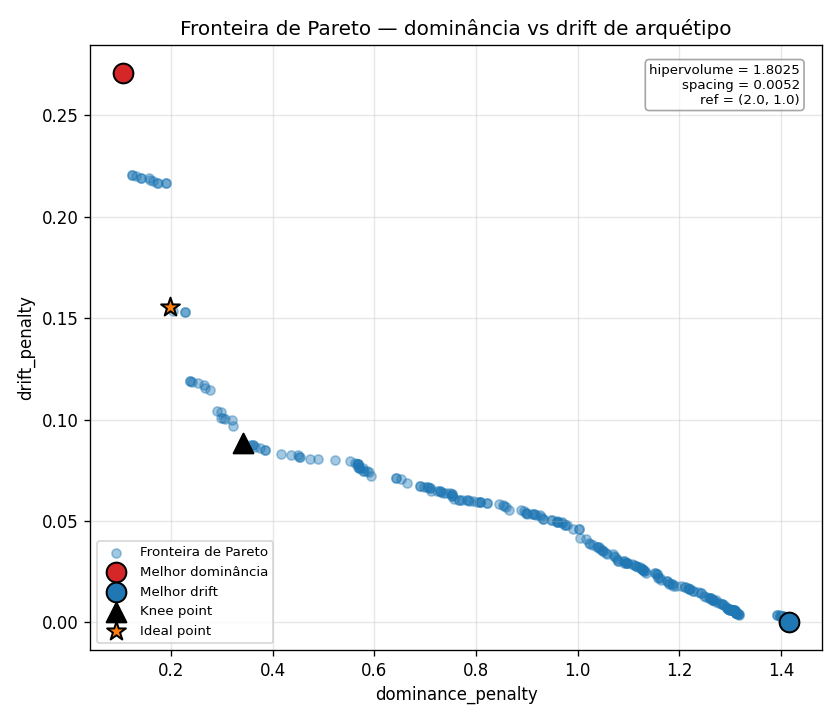
\includegraphics[width=\columnwidth]{pareto_front.png}
\caption{Fronteira de Pareto (desbalanço $\times$ desvio) obtida pelo NSGA-II. Cada
ponto é um \emph{roster} não dominado; os destacados marcam os extremos, o
\emph{knee point} e o \emph{ideal point}.}
\label{fig:pareto}
\end{figure}

A Tabela~\ref{tab:tradeoff} resume quatro pontos do \emph{trade-off}. No extremo de
identidade perfeita (canônico, que coincide com \emph{best\_drift}), o equilíbrio é
nulo. No ponto do AG escalar, o equilíbrio é total, mas a identidade se erode. O
\emph{knee\_point} ocupa a posição intermediária: reduz o desbalanço de $\domCan{}$
para $\domKnee{}$ --- três quartos do caminho --- preservando \valKnee{} das
\valTotal{} asserções, ainda que apenas \eqKnee{} dos dez pares caiam na banda
estrita de $[40\%,60\%]$; seu ganho é sobretudo de equilíbrio \emph{global}, não par
a par. Já o \emph{best\_dominance} leva o equilíbrio quase ao limite: pagando um
desvio de $\driftBd{}$, atinge \eqBd{} dos dez confrontos equilibrados, com um único
\emph{hard-counter}, mas o validador cai para \valBd{} de \valTotal{} --- ainda que a
diferenciação par a par permaneça em $\diffBd{}$, acima do $\diffAg{}$ do AG escalar,
indicando homogeneização modesta. Quanto ao ciclo canônico, não codificado na função
objetivo: ele se mantém em \cycleCan{} a \cycleBd{} dos dez pares em \emph{todos} os
pontos da tabela --- a evolução não o destrói, mas tampouco o recupera.

\begin{table}[!t]
\renewcommand{\arraystretch}{1.15}
\setlength{\tabcolsep}{4pt}
\caption{Quatro Pontos do \emph{Trade-off} Equilíbrio $\times$ Identidade}
\label{tab:tradeoff}
\centering
\footnotesize
\begin{tabular}{lcccc}
\toprule
Métrica & Canôn. & AG esc. & Joelho & Equilíb. \\
\midrule
\emph{dominance} $\downarrow$   & \domCan   & \domAg   & \domKnee   & \domBd \\
\emph{drift} $\downarrow$       & \driftCan & \driftAg & \driftKnee & \driftBd \\
Confrontos eq.\ (de 10)         & \eqCan    & \eqAg    & \eqKnee    & \eqBd \\
Diferenciação                   & \diffCan  & \diffAg  & \diffKnee  & \diffBd \\
Validador (de \valTotal)        & \valCan   & \valAg   & \valKnee   & \valBd \\
Ciclo (de \cycleTotal)          & \cycleCan & \cycleAg & \cycleKnee & \cycleBd \\
\bottomrule
\end{tabular}
\vspace{2pt}
\footnotesize
\raggedright
\emph{Confrontos eq.}: pares com taxa de vitória em $[40\%,60\%]$.
\emph{Diferenciação}: razão da distância média par a par vs.\ o canônico ($<1$ =
homogeneização). \emph{Joelho} e \emph{Equilíb.}: representantes
\emph{knee\_point} e \emph{best\_dominance} da fronteira; o canônico coincide com
\emph{best\_drift}.
\end{table}

Sobre \nSeeds{} execuções independentes, o NSGA-II aterrissa em
$\textit{dominance}=\aggDomMean{}\pm\aggDomStd{}$ e
$\textit{drift}=\aggDriftMean{}\pm\aggDriftStd{}$; o equilíbrio \emph{global} é a
parte estrutural (cada personagem equilibrado em 90--100\% das execuções), enquanto
zerar todos os \emph{hard-counters} de par é sensível à semente
($\hcPerSeed{}\pm\hcPerSeedStd{}$ pares residuais por execução). Sob \extNSeeds{}
sementes novas, fora do laço, \robBd{} dos \robTotal{} confrontos seguem
equilibrados: o equilíbrio reportado \textbf{não é} artefato de sobreajuste.

\section{Conclusões}

Os resultados preliminares sustentam uma resposta afirmativa, ainda que matizada: o
equilíbrio competitivo \emph{pode} ser alcançado sem destruir as identidades
funcionais, mas sob um \emph{trade-off} mensurável --- o grau de equilíbrio buscado
determina quanto de identidade se preserva. O equilíbrio substancial (\eqBd{}
confrontos) preserva a diferenciação par a par ($\diffBd{}$), embora o validador
estrutural caia para \valBd{} de \valTotal{}: a identidade se erode nos
ranqueamentos antes de se dissolver na geometria do elenco --- e o equilíbrio total
(\eqAg{}) custa mais, com o validador em \valAg{}. A separação entre objetivos
otimizados e métricas \emph{post hoc} é o que sustenta a não circularidade dessa
resposta.

Três delimitações balizam o alcance dos resultados. O modelo simplifica os jogos de
luta reais --- não representa \emph{frames} de inicialização e recuperação,
\emph{mix-ups} nem oclusão ---, e o achado de que o ciclo canônico não sobrevive a
ele é evidência de que essas mecânicas têm papel estrutural. O estudo emprega cinco
arquétipos, ante os dez ou mais dos jogos reais. E o \emph{round-robin} pressupõe
todos jogados em igual proporção, sem modelar o \emph{matchmaking}.

Como trabalho em andamento, três frentes seguem abertas: a calibração final dos
limites dos genes e da banda de \emph{hard-counter}, hoje provisórios; o teste de
estresse do equilíbrio por coevolução \cite{chen2014mmorpg}, para verificar se ele
sobrevive a um oponente que também se adapta; e a reformulação por
\emph{quality-diversity} \cite{mouret2015mapelites}, que substituiria a busca por
uma única solução pela iluminação de \emph{quantas} configurações distintas de
\emph{roster} atingem equilíbrio.

\section*{Agradecimentos}

Os autores agradecem ao orientador e à instituição de ensino pelo apoio ao
desenvolvimento deste trabalho. \ph{completar com nomes e afiliação na versão
final, após o aceite}

\section*{Declaração sobre uso de Inteligência Artificial}

Declaramos que ferramentas de Inteligência Artificial Generativa foram utilizadas
neste trabalho nas seguintes etapas: Claude (Anthropic) como assistente de
programação na implementação do simulador de combate, dos algoritmos evolutivos e
das ferramentas de análise (desenvolvimento do sistema), e no apoio à redação e
revisão do texto (escrita); Claude (Anthropic) e ChatGPT (OpenAI) no levantamento e
triagem de referências bibliográficas (fundamentação teórica). Todo o conteúdo
gerado foi revisado criticamente e validado pelos autores,
que assumem integral responsabilidade pela originalidade e veracidade do texto
final, em conformidade com a Portaria CNPq n\textsuperscript{o} 2.664/2026.

\bibliographystyle{IEEEtran}
\bibliography{referencias}

\end{document}
